\subsection*{(a)}
\FloatBarrier
We compute the speedup $\frac{T_1}{T_p}$ for different combinations of non-parallelizable fractions of code and the number of processors in \Cref{tab:ex1}. The graph of the cross section along the middle row is found in \Cref{FixProc} and the graph of the cross section along the middle column is found in \Cref{FixFrac}. We choose to evaluate the Speedup in the number of processors in an exponential scale, since for a large number of processors, relatively small changes become less important. On the other hand, we choose equally spaced $a$, since the whole range seems interesting.
\\

The results of this exercise give us a realistic expectation of what to expect from the speedups possible with parallelization. We see in \Cref{FixProc} that it highly depends on the fraction of parallelizable code and that already a little fraction of non-parallelizable code is enough to strongly dampen the speedup. Also, in \Cref{FixFrac} we see that given a fixed fraction of non-parallelizable code, it does not make sense to increase the number of processors at some point as the speedup converges asyptotically to a maximum given through Amdahl's law. The overall conclusion is that it is crucial to develop algorithms with an as large as possible parallelizable fraction to see the benefits of parallel computing and that the latter is not a magic tool that makes every computation efficient.


\begin{table}[h]
\hspace{-0.1cm}
\begin{tabular}{|c|c|c|c|c|c|c|c|c|c|c|c|}
\hline
\diagbox[innerwidth = 2cm, height = 3ex]{p}{a} & $0$ & $0.1$ & $0.2$ & $0.3$ & $0.4$ & $0.5$ & $0.6$ & $0.7$ & $0.8$ & $0.9$ & $1$\\ 
\hline 
$1$ & $1$ & $1$ & $1$ & $1$ & $1$ & $1$ & $1$ & $1$ & $1$ & $1$ & $1$ \\ 
\hline 
$2$ & $2$ & $1.818$ & $1.666$ & $1.538$ & $1.428$ & $1.333$ & $1.25$ & $1.176$ & $1.111$ & $1.052$ & $1$ \\ 
\hline 
$4$ & $4$ & $3.076$ & $2.5$ & $2.105$ & $1.818$ & $1.6$ & $1.428$ & $1.29$ & $1.176$ & $1.081$ & $1$ \\ 
\hline 
$8$ & $8$ & $4.705$ & $3.333$ & $2.58$ & $2.105$ & $1.777$ & $1.538$ & $1.355$ & $1.212$ & $1.095$ & $1$ \\ 
\hline 
$16$ & $16$ & $6.4$ & $4$ & $2.909$ & $2.285$ & $1.882$ & $1.6$ & $1.391$ & $1.23$ & $1.103$ & $1$ \\ 
\hline 
$32$ & $32$ & $7.804$ & $4.444$ & $3.106$ & $2.388$ & $1.939$ & $1.632$ & $1.409$ & $1.24$ & $1.107$ & $1$ \\ 
\hline 
$64$ & $64$ & $8.767$ & $4.705$ & $3.216$ & $2.442$ & $1.969$ & $1.649$ & $1.419$ & $1.245$ & $1.109$ & $1$ \\ 
\hline 
$128$ & $128$ & $9.343$ & $4.848$ & $3.273$ & $2.471$ & $1.984$ & $1.658$ & $1.423$ & $1.247$ & $1.11$ & $1$ \\ 
\hline 
$256$ & $256$ & $9.66$ & $4.923$ & $3.303$ & $2.485$ & $1.992$ & $1.662$ & $1.426$ & $1.248$ & $1.110$ & $1$ \\ 
\hline 
$512$ & $512$ & $9.827$ & $4.961$ & $3.318$ & $2.492$ & $1.996$ & $1.664$ & $1.427$ & $1.249$ & $1.11$ & $1$ \\ 
\hline 
$1024$ & $1024$ & $9.912$ & $4.98$ & $3.325$ & $2.496$ & $1.998$ & $1.665$ & $1.427$ & $1.249$ & $1.11$ & $1$ \\ 
\hline 
\end{tabular}
\caption{Speedups for different combinations of non-parallelizable fractions and processor numbers}
\label{tab:ex1}
\end{table}


\begin{figure}[h]
\centering
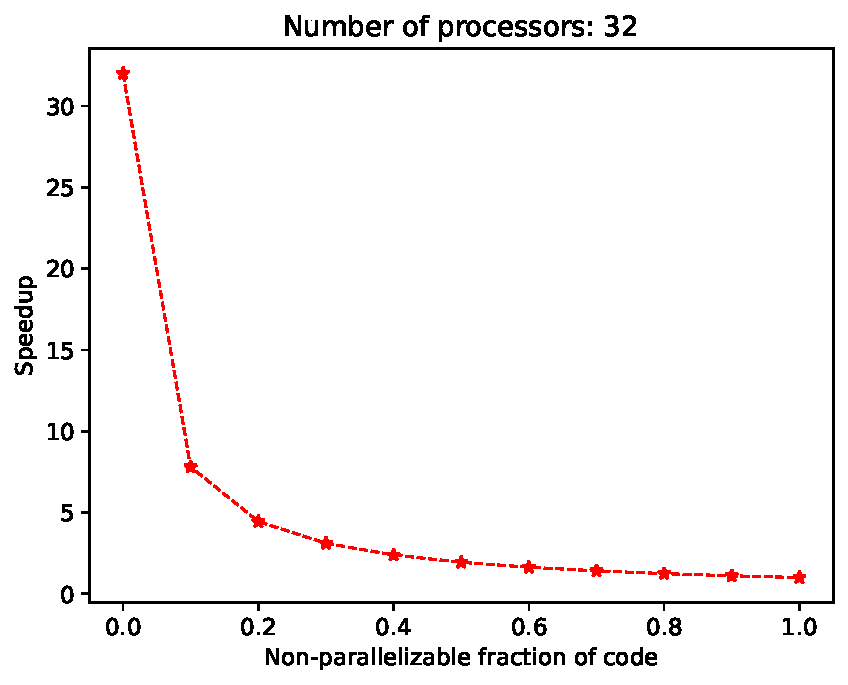
\includegraphics[width=0.9\textwidth]{FixProc.pdf}
\caption{Speedup for a fixed number of processors over the fraction of non-parallelizable code}
\label{FixProc}
\end{figure}

\begin{figure}[h]
\centering
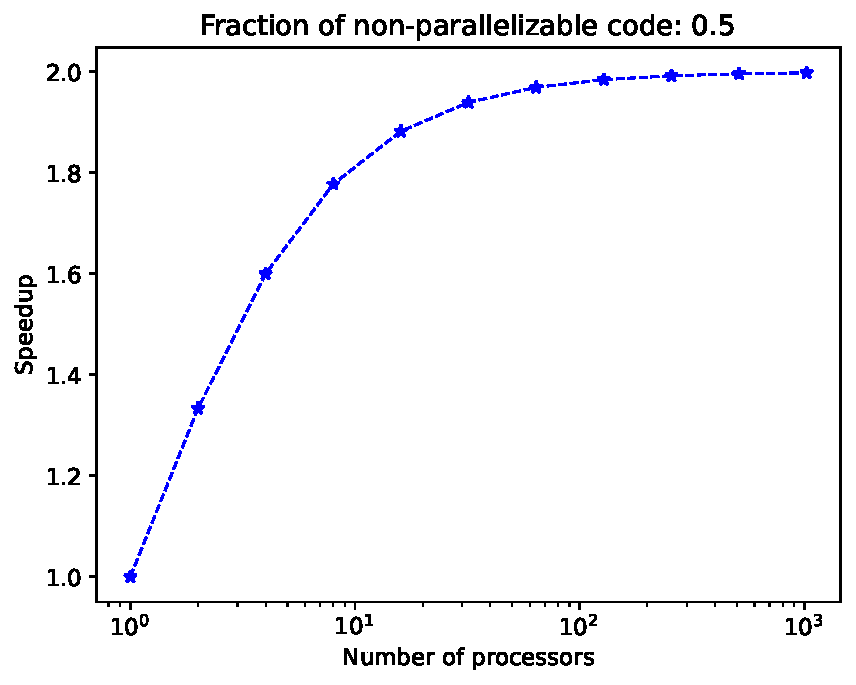
\includegraphics[width=0.9\textwidth]{FixFrac.pdf}
\caption{Speedup for a fixed fraction of non-parallelizable code over the number of processors}
\label{FixFrac}
\end{figure}



\begin{comment}
[0.  0.1 0.2 0.3 0.4 0.5 0.6 0.7 0.8 0.9 1. ]
[   1    2    4    8   16   32   64  128  256  512 1024]
[[1.00000000e+00 1.00000000e+00 1.00000000e+00 1.00000000e+00
  1.00000000e+00 1.00000000e+00 1.00000000e+00 1.00000000e+00
  1.00000000e+00 1.00000000e+00 1.00000000e+00]
 [2.00000000e+00 1.81818182e+00 1.66666667e+00 1.53846154e+00
  1.42857143e+00 1.33333333e+00 1.25000000e+00 1.17647059e+00
  1.11111111e+00 1.05263158e+00 1.00000000e+00]
 [4.00000000e+00 3.07692308e+00 2.50000000e+00 2.10526316e+00
  1.81818182e+00 1.60000000e+00 1.42857143e+00 1.29032258e+00
  1.17647059e+00 1.08108108e+00 1.00000000e+00]
 [8.00000000e+00 4.70588235e+00 3.33333333e+00 2.58064516e+00
  2.10526316e+00 1.77777778e+00 1.53846154e+00 1.35593220e+00
  1.21212121e+00 1.09589041e+00 1.00000000e+00]
 [1.60000000e+01 6.40000000e+00 4.00000000e+00 2.90909091e+00
  2.28571429e+00 1.88235294e+00 1.60000000e+00 1.39130435e+00
  1.23076923e+00 1.10344828e+00 1.00000000e+00]
 [3.20000000e+01 7.80487805e+00 4.44444444e+00 3.10679612e+00
  2.38805970e+00 1.93939394e+00 1.63265306e+00 1.40969163e+00
  1.24031008e+00 1.10726644e+00 1.00000000e+00]
 [6.40000000e+01 8.76712329e+00 4.70588235e+00 3.21608040e+00
  2.44274809e+00 1.96923077e+00 1.64948454e+00 1.41906874e+00
  1.24513619e+00 1.10918544e+00 1.00000000e+00]
 [1.28000000e+02 9.34306569e+00 4.84848485e+00 3.27365729e+00
  2.47104247e+00 1.98449612e+00 1.65803109e+00 1.42380423e+00
  1.24756335e+00 1.11014744e+00 1.00000000e+00]
 [2.56000000e+02 9.66037736e+00 4.92307692e+00 3.30322581e+00
  2.48543689e+00 1.99221790e+00 1.66233766e+00 1.42618384e+00
  1.24878049e+00 1.11062907e+00 1.00000000e+00]
 [5.12000000e+02 9.82725528e+00 4.96124031e+00 3.31821128e+00
  2.49269718e+00 1.99610136e+00 1.66449935e+00 1.42737664e+00
  1.24938995e+00 1.11087004e+00 1.00000000e+00]
  
  
 [1.02400000e+03 9.91287512e+00 4.98054475e+00 3.32575512e+00
  2.49634325e+00 1.99804878e+00 1.66558230e+00 1.42797378e+00
  1.24969490e+00 1.11099056e+00 1.00000000e+00]]
  \end{comment}
  
  \FloatBarrier
  
  
  
\subsection*{(b)}
\FloatBarrier
When $a$ is the fraction of non-parallelizable code, Ahmdals law describes the time $T_p$ to run on $p$ processors as
\[
T_P = (1 - a)\frac{T_1}{p} + a T_1,
\]
where $T_1$ is the time needed to solve the problem on $1$ node and $p$ is the number of nodes. A computation derives the parallel efficiency as
\begin{align*}
	E & = \frac{T_1}{pT_p} = \frac{T_1}{p(1 - a)\frac{T_1}{p} + ap T_1} = \frac{1}{1 - a + ap}.
\end{align*}
\FloatBarrier

\subsection*{(c)}
\FloatBarrier
As an example we can consider the method of lines for the solution $u(x, t)$ of a scalar hyperbolic PDE with two dimensional space component $x \in \Omega \subset \R^2$ and one dimensional time component $t$. Due to finite speed of information propagation, coming from hyperbolicity, it is enough to use $\Delta t = \Ocal(\Delta x)$ to ensure stability. We can and will therefore assume for now that $\Delta x = \Ocal(\frac{1}{n})$ and $\Delta t = \Ocal\left(\frac{1}{n}\right)$. Put simply, the method of lines discretizes space and computes the time update through independent ODEs. The cost for computing these updates with Euler's method is $\Ocal\left(\frac{1}{\Delta t}\right) = \Ocal(n)$. Further, this time update is a sequential operation that is not parallelizable. Since space is two dimensional here, this has to be done independently $\Ocal\left(\frac{1}{(\Delta x)^2}\right) = \Ocal(n^2)$ times, once at each grid point. This can be done completely in parallel. Concluding, the overall cost of the problem grows as
\[
\Ocal(n^2) \cdot \Ocal(n) = \Ocal(n^3),
\]
whereas the non-parallelizable part of it grows as
\[
\Ocal(n).
\]
Translating this into the language of the previous parts, the non-paralellizable fraction $a$ evolves as
\[
a = \Ocal\left(\frac{n}{n^3}\right) = \Ocal\left(\frac{1}{n^2}\right),
\]
and the parallelizable fraction evolves as
\[
1 - a = \Ocal\left(1 - \frac{1}{n^2}\right).
\]
Choosing an appropriate $p = \Ocal(n^2)$ gives here constant parallel efficiency.
\FloatBarrier

\subsection*{(d)}
\FloatBarrier
Let all the notions be given as in the exercise sheet. We assume that the time necessary to solve the problem without parallelization is $T_1$. The time $T_P$ to run on the maximal number of nodes is then given by summing the parallelized runtimes for the different classes of work:
\[
T_P = \sum_{p = 1}^P a_p \frac{T_1}{p},
\]
The respective speedup is given by
\[
\frac{T_1}{T_P} = \frac{1}{\sum_{p = 1}^P \frac{a_p}{p}}.
\]
\FloatBarrier
  
  
  
  
  
  
  
  
  
  
  
  
  
  
  
  
  
  
  
  
  
  
  
  
  
  
  
  
  
  
  
  
  
  
  
  
  
  
  
  
  
  
  
  
  
  
  
  
  
  
  